% move all configuration stuff into one file so we can focus on the content
\documentclass[aspectratio=169,hyperref={pdfpagelabels=false,colorlinks=true,linkcolor=white,urlcolor=lightblue},xcolor={table},t]{beamer}

%%%%%%%%%%%%%%%%%%%%%%%%%%%%%%%%%%%%%%%%%%%%%%%%%%%%%%%%%%%%%%%%%%%%%%%%%%%%%%%%%%
%%%%%%%%%%%%%%%%%%%%%%%%%%%%%%%%%%%%%%%%%%%%%%%%%%%%%%%%%%%%%%%%%%%%%%%%%%%%%%%%%%
% packages
\usepackage{pict2e}
\usepackage{epic}
\usepackage{amsmath,amsfonts,amssymb}
\usepackage{units}
\usepackage{fancybox}
\usepackage[absolute,overlay]{textpos} 
%\usepackage[table]{xcolor}
\usepackage{animate}
\usepackage{gensymb}
%\usepackage{graphicx}
%\usepackage{longtable}
\usepackage{multirow}
\usepackage{silence}
\usepackage{tikz}
\usepackage[backend=bibtex,style=ieee]{biblatex}
\AtEveryCitekey{\iffootnote{\tiny}{}}
%\addbibresource{include/references}



% fontsize
\let\Tiny=\tiny

%%%%%%%%%%%%%%%%%%%%%%%%%%%%%%%%%%%%%%%%%%%%%%%%%%%%%%%%%%%%%%%%%%%%%%%%%%%%%%%%%%
%%%%%%%%%%%%%%%%%%%%%%%%%%%%%%%%%%%%%%%%%%%%%%%%%%%%%%%%%%%%%%%%%%%%%%%%%%%%%%%%%%
% warnings
\pdfsuppresswarningpagegroup=1
\WarningFilter{biblatex}{Patching footnotes failed}
\WarningFilter{latexfont}{Font shape}
\WarningFilter{latexfont}{Some font shapes}
\WarningFilter{gensymb}{Not defining}


%%%%%%%%%%%%%%%%%%%%%%%%%%%%%%%%%%%%%%%%%%%%%%%%%%%%%%%%%%%%%%%%%%%%%%%%%%%%%%%%%%
%%%%%%%%%%%%%%%%%%%%%%%%%%%%%%%%%%%%%%%%%%%%%%%%%%%%%%%%%%%%%%%%%%%%%%%%%%%%%%%%%%
% colors
\definecolor{gtgold}{rgb}{.914, .664, 0} %0e7eed {rgb}{0.88,0.66,1,0.06} [234, 170, 0]/256 %96caff
\definecolor{darkgray}{rgb}{.15, .15, .15}
\definecolor{lightblue}{HTML}{0e7eed}
\definecolor{highlight}{rgb}{0, 0, 1} %_less!40

%%%%%%%%%%%%%%%%%%%%%%%%%%%%%%%%%%%%%%%%%%%%%%%%%%%%%%%%%%%%%%%%%%%%%%%%%%%%%%%%%%
%%%%%%%%%%%%%%%%%%%%%%%%%%%%%%%%%%%%%%%%%%%%%%%%%%%%%%%%%%%%%%%%%%%%%%%%%%%%%%%%%%
% relative paths
\graphicspath{{../graph/}}


%%%%%%%%%%%%%%%%%%%%%%%%%%%%%%%%%%%%%%%%%%%%%%%%%%%%%%%%%%%%%%%%%%%%%%%%%%%%%%%%%%
%%%%%%%%%%%%%%%%%%%%%%%%%%%%%%%%%%%%%%%%%%%%%%%%%%%%%%%%%%%%%%%%%%%%%%%%%%%%%%%%%%
% units
\setlength{\unitlength}{1mm}

%%%%%%%%%%%%%%%%%%%%%%%%%%%%%%%%%%%%%%%%%%%%%%%%%%%%%%%%%%%%%%%%%%%%%%%%%%%%%%%%%%
%%%%%%%%%%%%%%%%%%%%%%%%%%%%%%%%%%%%%%%%%%%%%%%%%%%%%%%%%%%%%%%%%%%%%%%%%%%%%%%%%%
% math
\DeclareMathOperator*{\argmax}{argmax}
\DeclareMathOperator*{\argmin}{argmin}
\DeclareMathOperator*{\atan}{atan}
\DeclareMathOperator*{\arcsinh}{arcsinh}
\DeclareMathOperator*{\sign}{sign}
\DeclareMathOperator*{\tcdf}{tcdf}
\DeclareMathOperator*{\si}{sinc}
\DeclareMathOperator*{\princarg}{princarg}
\DeclareMathOperator*{\arccosh}{arccosh}
\DeclareMathOperator*{\hwr}{HWR}
\DeclareMathOperator*{\flip}{flip}
\DeclareMathOperator*{\sinc}{sinc}
\DeclareMathOperator*{\floor}{floor}
\newcommand{\e}{{e}}
\newcommand{\jom}{\mathrm{j}\omega}
\newcommand{\jOm}{\mathrm{j}\Omega}
\newcommand   {\mat}[1]    		{\boldsymbol{\uppercase{#1}}}		%bold
\renewcommand {\vec}[1]    		{\boldsymbol{\lowercase{#1}}}		%bold

%%%%%%%%%%%%%%%%%%%%%%%%%%%%%%%%%%%%%%%%%%%%%%%%%%%%%%%%%%%%%%%%%%%%%%%%%%%%%%%%%%
%%%%%%%%%%%%%%%%%%%%%%%%%%%%%%%%%%%%%%%%%%%%%%%%%%%%%%%%%%%%%%%%%%%%%%%%%%%%%%%%%%
% media9
\newcommand{\includeaudio}[1]{
\href{run:audio/#1.mp3}{
\includegraphics[width=5mm, height=5mm]{graph/SpeakerIcon}}}

\newcommand{\includeanimation}[4]{{\begin{center}
                        \animategraphics[autoplay,loop,scale=.7]{#4}{animation/#1-}{#2}{#3}        
                        \end{center}
                        \addreference{matlab source: \href{https://github.com/alexanderlerch/ACA-Plots/blob/master/matlab/animate#1.m}{matlab/animate#1.m}}}
                        \inserticon{video}}
                        
%%%%%%%%%%%%%%%%%%%%%%%%%%%%%%%%%%%%%%%%%%%%%%%%%%%%%%%%%%%%%%%%%%%%%%%%%%%%%%%%%%
%%%%%%%%%%%%%%%%%%%%%%%%%%%%%%%%%%%%%%%%%%%%%%%%%%%%%%%%%%%%%%%%%%%%%%%%%%%%%%%%%%
% other commands
\newcommand{\question}[1]{%\vspace{-4mm}
                          \setbeamercovered{invisible}
                          \begin{columns}[T]
                            \column{.9\textwidth}
                                \textbf{#1}
                            \column{.1\textwidth}
                                \vspace{-8mm}
                                \begin{flushright}
                                     
\includegraphics[width=.9\columnwidth]{graph/question_mark}
                                \end{flushright}
                                \vspace{6mm}
                          \end{columns}\pause\vspace{-12mm}}

\newcommand{\toremember}[1]{
                        \inserticon{lightbulb}
                        }

\newcommand{\matlabexercise}[1]{%\vspace{-4mm}
                          \setbeamercovered{invisible}
                          \begin{columns}[T]
                            \column{.8\textwidth}
                                \textbf{matlab exercise}: #1
                            \column{.2\textwidth}
                                \begin{flushright}
                                     \includegraphics[scale=.5]{graph/logo_matlab}
                                \end{flushright}
                                %\vspace{6mm}
                          \end{columns}}

\newcommand{\addreference}[1]{  
                  
                    \begin{textblock*}{\baselineskip }(.98\paperwidth,.5\textheight) %(1.15\textwidth,.4\textheight)
                         \begin{minipage}[b][.5\paperheight][b]{1cm}%
                            \vfill%
                             \rotatebox{90}{\tiny {#1}}
                        \end{minipage}
                   \end{textblock*}
                    }
                    
\newcommand{\figwithmatlab}[1]{
                    \begin{figure}
                        \centering
                        \includegraphics[scale=.7]{#1}
                        %\label{fig:#1}
                    \end{figure}
                    
                    \addreference{matlab source: \href{https://github.com/alexanderlerch/MUSI-6202/blob/main/matlab/plot#1.m}{plot#1.m}}}
\newcommand{\figwithref}[2]{
                    \begin{figure}
                        \centering
                        \includegraphics[scale=.7]{#1}
                        \label{fig:#1}
                    \end{figure}
                    
                    \addreference{#2}}  
                                    
\newcommand{\inserticon}[1]{
                    \begin{textblock*}{100mm}(14.5cm,7.5cm)
                        \includegraphics[height=.8cm,keepaspectratio]{graph/#1}
                    \end{textblock*}}            

%%%%%%%%%%%%%%%%%%%%%%%%%%%%%%%%%%%%%%%%%%%%%%%%%%%%%%%%%%%%%%%%%%%%%%%%%%%%%%%%%%
%%%%%%%%%%%%%%%%%%%%%%%%%%%%%%%%%%%%%%%%%%%%%%%%%%%%%%%%%%%%%%%%%%%%%%%%%%%%%%%%%%
% counters
\newcounter{i}
\newcounter{j}
\newcounter{iXOffset}
\newcounter{iYOffset}
\newcounter{iXBlockSize}
\newcounter{iYBlockSize}
\newcounter{iYBlockSizeDiv2}
\newcounter{iXBlockSizeDiv2}
\newcounter{iDistance}

\newcommand{\IEEELink}{https://ieeexplore.ieee.org/servlet/opac?bknumber=9965970}



\subtitle{Part 13: Digital Number Formats}

%%%%%%%%%%%%%%%%%%%%%%%%%%%%%%%%%%%%%%%%%%%%%%%%%%%%%%%%%%%%%%%%%%%%%%%%%%%%
\begin{document}
    % generate title page
	\title[]{Digital Signal Processing for Music}   
\author[alexander lerch]{alexander lerch} 
%\institute{~}
%\date[Alexander Lerch]{}
\titlegraphic{\vspace{-16mm}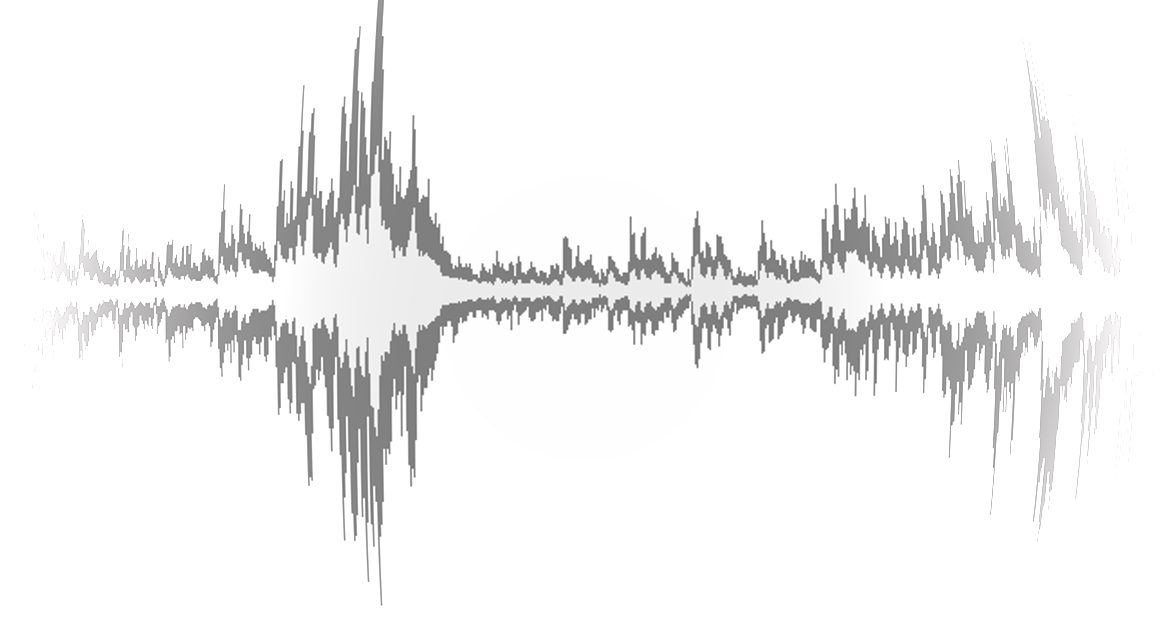
\includegraphics[width=\textwidth,height=3cm]{title}}


\begin{frame}
    \titlepage
    %\vspace{-5mm}
    \begin{flushright}
        \href{http://www.gtcmt.gatech.edu}{
\includegraphics[height=.8cm,keepaspectratio]{../shared/Logo_GTCMT_black}}
    \end{flushright}
\end{frame}


\section[intro]{introduction}

	\begin{frame}{number formats}{word length and SNR}
			\begin{table}
			\centering
				\begin{footnotesize}
					\begin{tabular}{lccc}
					\hline
						\textbf{w} & \textbf{$\Delta$} & \textbf{Max.\ Amp} & \textbf{theo.\ SNR} \\
					\hline
						8 (Int)	&	$\pm1$ & $0\ldots255$ & $\approx$\unit[48]{dB}\\
						16 (Int)	&	$\pm1$ & $-32768\ldots32767$ & $\approx$\unit[96]{dB}\\
						20 (Int)	&	$\pm1$ & $-524288\ldots524287$ & $\approx$\unit[120]{dB}\\
						24 (Int)	&	$\pm1$ & $-16777216\ldots16777215$ & $\approx$\unit[144]{dB}\\
					\hline
						32 (Float)	&	$\pm1.175\cdot10^{-38}$ & $\pm3.403\cdot10^{1038}$ & \unit[1529]{dB}\\
						64 (Float)	&	$\pm2.225\cdot10^{-308}$ & $\pm1.798\cdot10^{10308}$ & \unit[12318]{dB}\\
					\hline
					\end{tabular}  
				\end{footnotesize}
			\end{table}
            
            \bigskip
            \bigskip
            \question{how do we represent this in bits}
	\end{frame}	

\section[range]{value range}
	\begin{frame}{number formats}{value range}
		
            
			\begin{itemize}
				\item	\textbf{unnormalized}\footnote{remember: non-symmetric step count for positive and negative values}: $-2^{w-1}\ldots 2^{w-1}-1$
                    \begin{itemize}
                        \item   used for transmission etc.
                    \end{itemize}
				\bigskip
                \item	\textbf{normalized} (word length independent): $-1\ldots 1$
                    \begin{itemize}
                        \item   used for floating point representation
                        \item   used for processing
                    \end{itemize}
			\end{itemize}
            
            
	\end{frame}	

\section[number representation]{number representation}
	\begin{frame}{number formats}{number representation 1/2}
	    \begin{figure}
			\centering
				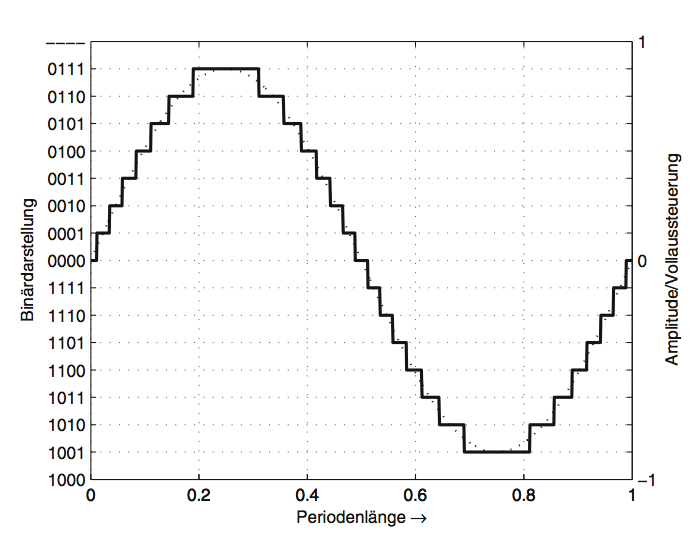
\includegraphics[scale=0.6]{Graph/2complement}
		\end{figure}
		\begin{itemize}
			\item	Least Significant Bit (LSB): $b_0$ (usually on the right)
			\item	Most Significant Bit (MSB): $b_{w-1}$ (usually on the left)
		\end{itemize}
	\end{frame}	

	\begin{frame}{number formats}{number representation 2/2}
		\begin{table}
			\centering
			\begin{footnotesize}
				\begin{tabular}{clc}
				\hline
				\textbf{format} & \textbf{amplitude} & \textbf{range (normalized)}\\
				\hline
				2-Complement & $x_Q = -b_{w-1} + \sum\limits_{i=0}^{w-2}b_{i}2^{-(w-i-1)}$ & $-1\leq x_Q \leq 1-2^{-(w-1)}$\\
				unsigned & $x_Q = \sum\limits_{i=0}^{w-1}b_i2^{-(w-1)}$ & $0\leq x_Q \leq 1-2^{-w}$\\
				\hline
				\end{tabular}
			\end{footnotesize}
		\end{table}
		\begin{itemize}
			\item	$w:$ word length
			\item	$b_i:$ ith Bit
		\end{itemize}
        \vspace{-10mm}
	    \begin{flushright}
			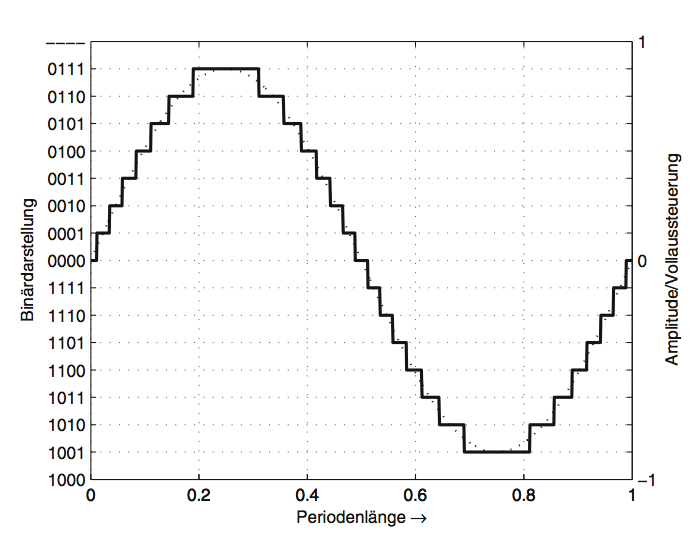
\includegraphics[scale=0.5]{Graph/2complement}
		\end{flushright}
	\end{frame}
	
\section[clipping]{clipping \& wrap-around}
	\begin{frame}{number formats}{quantization: clipping \& wrap-around}
        \begin{columns}
        \column{.9\linewidth}
	    \vspace{-10mm}
            \begin{figure}
                \centering
                    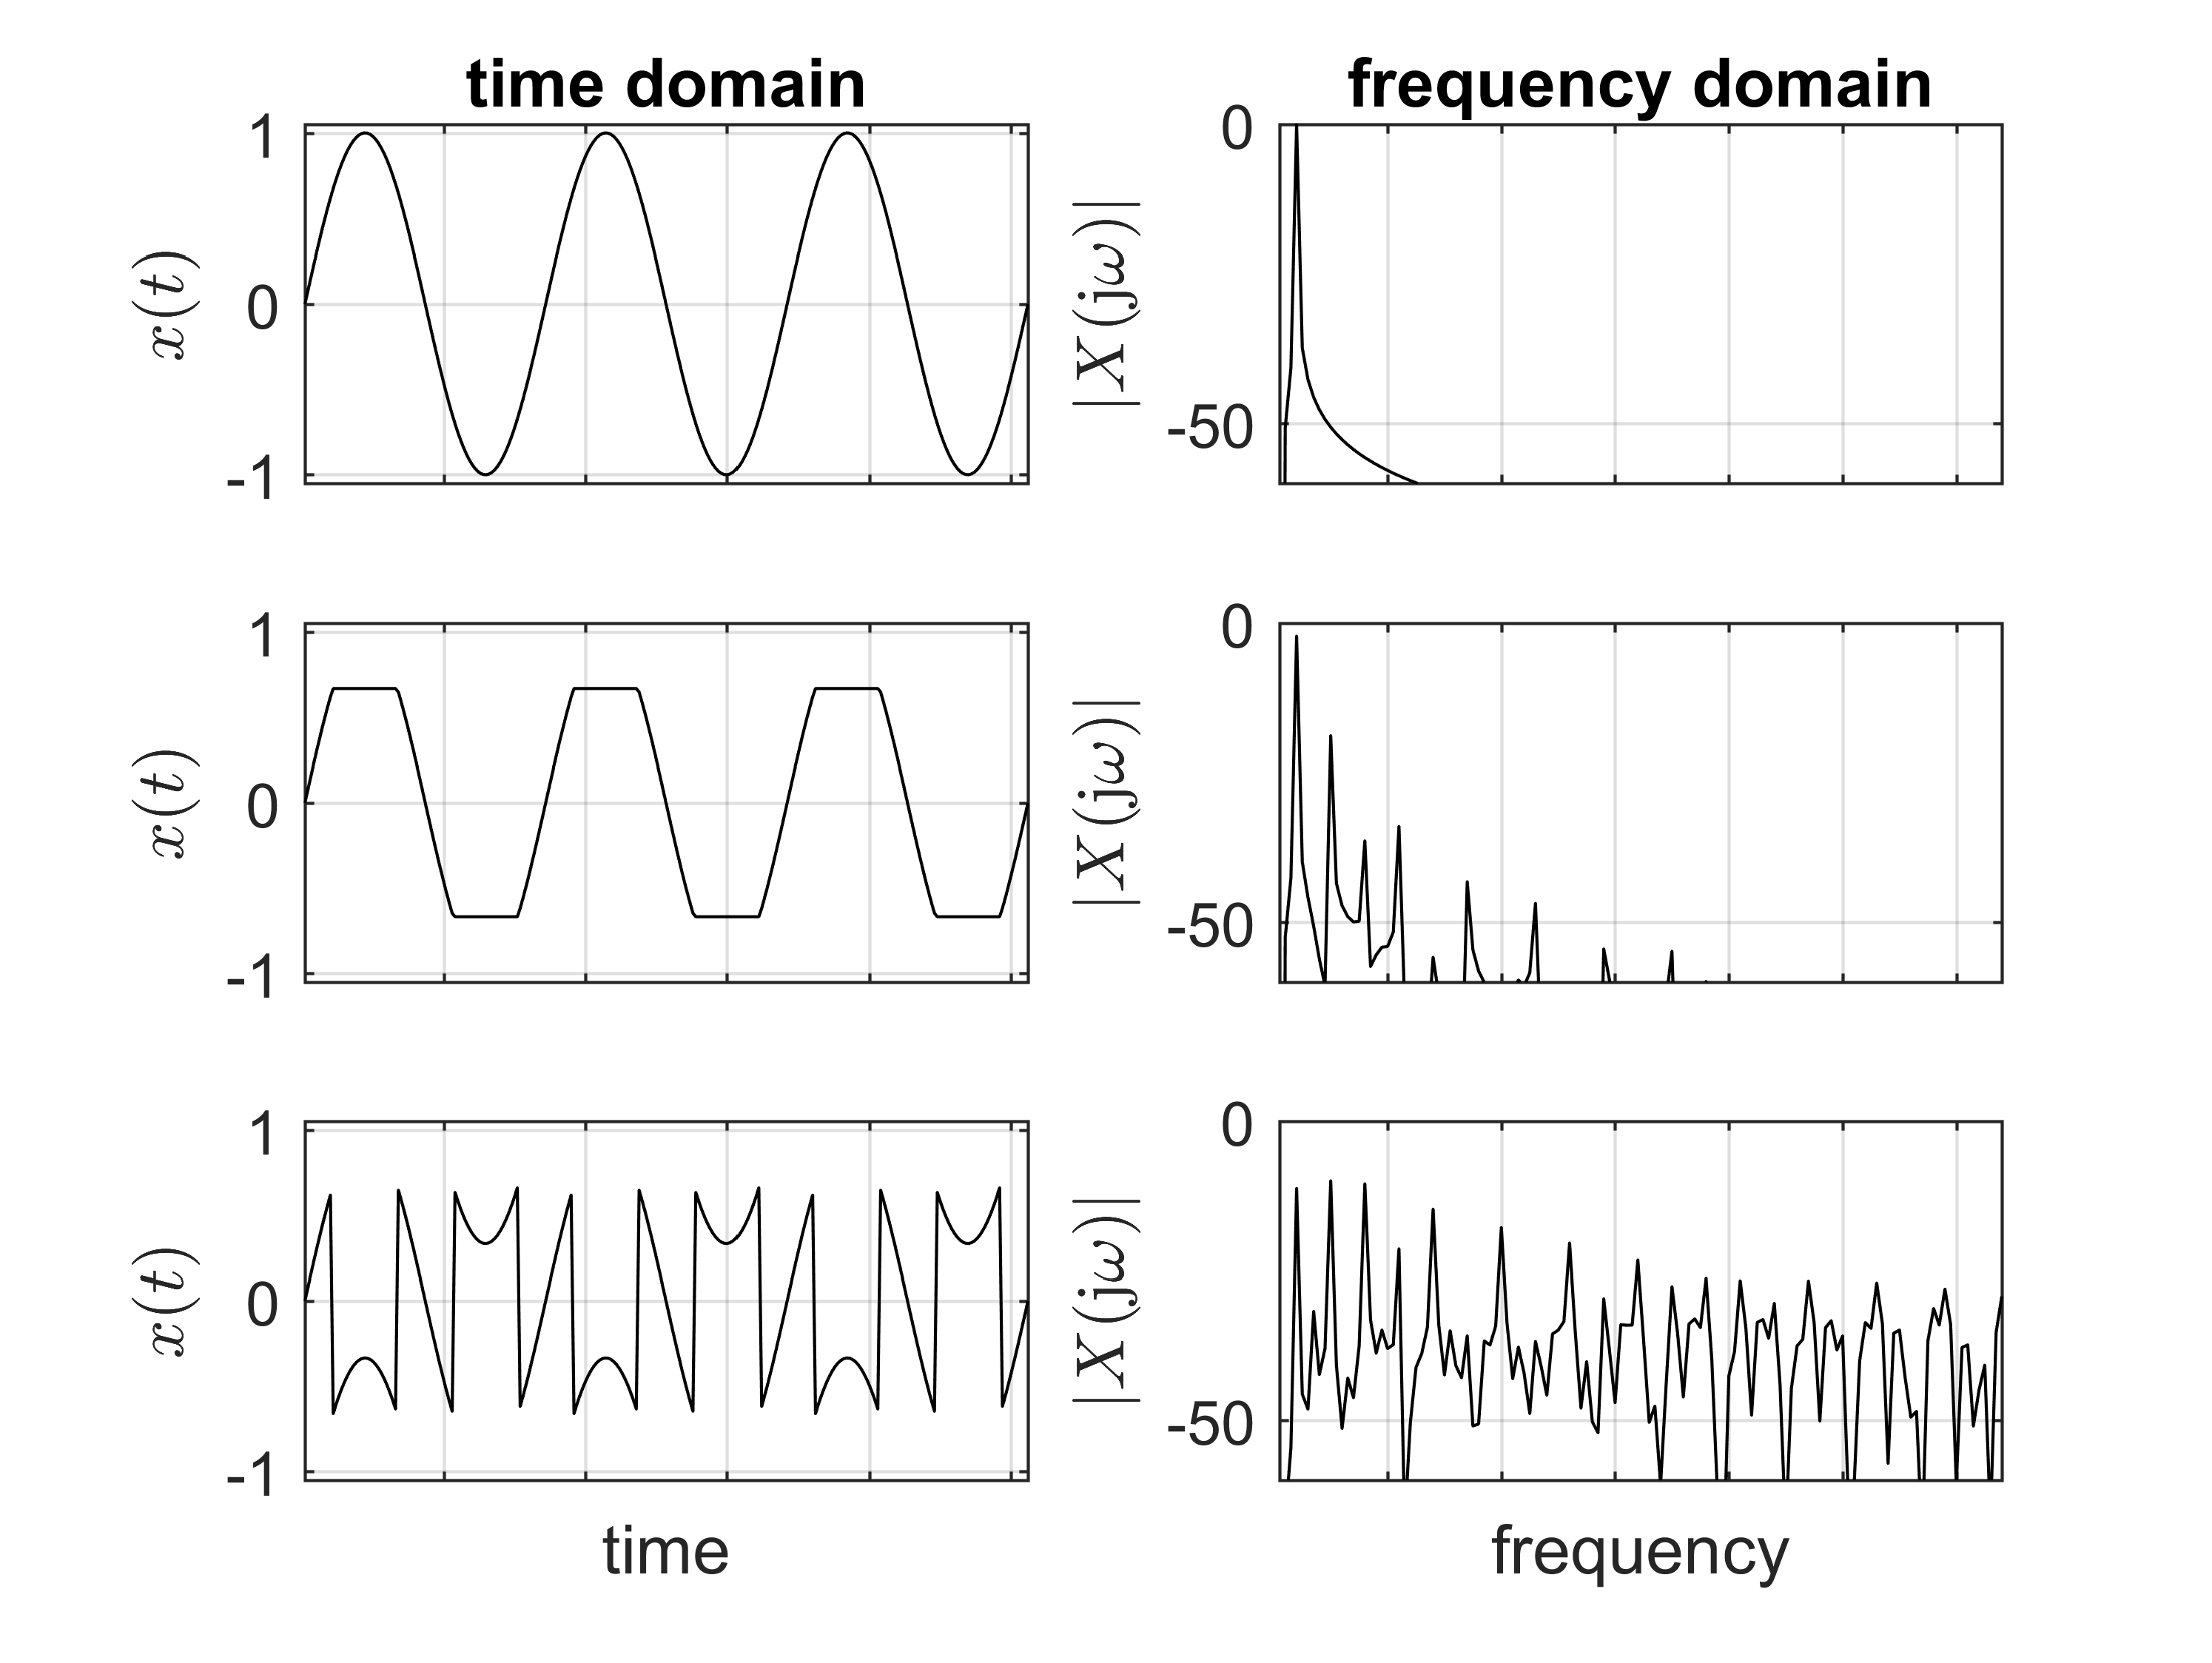
\includegraphics[scale=0.7]{Graph/wraparound}
            \end{figure}
        \column{.1\linewidth}
            %\vspace{5mm}
            
            \includeaudio{sine}
            \bigskip
            \bigskip
            \bigskip
            \bigskip
             
            \includeaudio{sine_clipped}
            \bigskip
            \bigskip
            \bigskip
            \bigskip
            
            \includeaudio{sine_wrapped}
        \end{columns}
	\end{frame}	
	
\section[fixed vs. float]{fixed point and floating point}
	\begin{frame}{number formats}{fixed point and floating point}
	
		number formats and their most frequent uses
		\begin{itemize}
			\item	\textbf{unsigned format}: small word lengths (4\ldots 8 Bit)
			\pause
			\item	\textbf{2's complement}: file formats with higher word lengths (16\ldots 24 Bit), some DSPs
			\pause
			\item	\only<4>{\textcolor{gtgold}}{\textbf{floating point}}: internal representation for processing
		\end{itemize}
	\end{frame}	
	
	\begin{frame}{number formats}{floating point 1/2}
		\begin{equation*}
		x_Q = M_G \cdot 2^{E_G}
		\end{equation*}
		
		\begin{itemize}
			\item	$M_G$: Normalized Mantissa $ 0.5 \leq M_{G} < 1$
			\item	$E_G$: Exponent
		\end{itemize}
		
		\pause
		\textbf{32 Bit IEEE 754 Floating Format}:
		\begin{table}
			\centering
			\begin{footnotesize}
				\begin{tabular}{ccc}
				\hline
				\textbf{Bit 31: Sign} & \textbf{Bits 30-23: Exponent} & \textbf{Bits 22-0: Mantissa}\\
				\hline
				$s$ & $e_{7}$ ... $e_{0}$ & $m_{22}$ ... $m_{0}$\\
				\hline
				\end{tabular}
			\end{footnotesize}
		\end{table}
		\pause
		\textit{Exceptions}
		\vspace{-3mm}
		\begin{table}
			\centering
			\begin{footnotesize}
					\begin{tabular}{cccl}
					\hline
					\textbf{Typ} & \textbf{$E_G$} & \textbf{$M_{G}$} & \textbf{Value}\\
					\hline 
					normal & $1\leq E_G \leq 254$ & any & $(-1)^s (0.m)2^{E_G-127}$\\
					\hline
					NAN (not a number)& 255 & $\neq 0$ & undefined\\
					\hline
					Infinity & 255 & $=0$ & $\infty$\\
					\hline
					Zero & 0 & 0 & 0\\
					\hline
					\end{tabular}
			\end{footnotesize}
		\end{table}
	\end{frame}	
	
	\begin{frame}{number formats}{floating point 2/2}
        \vspace{-5mm}
		\begin{columns}
			\column{5cm}
            \vspace{-3mm}
			\begin{figure}
				\centering
					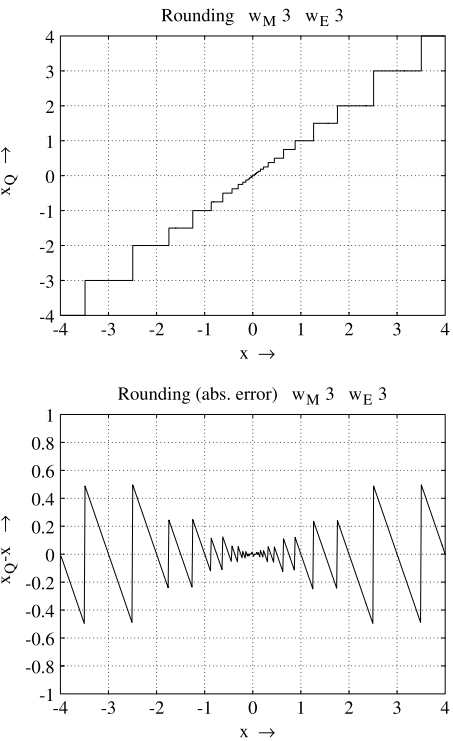
\includegraphics[scale=0.35]{Graph/floatquanterror}
			\end{figure}
			
			\column{4cm}
			\pause
			\begin{itemize}
				\item	\textbf{high exponent}: large quantization error energy
				\item	\textbf{low exponent}: small quantization error energy
			    \pause
                \bigskip
                \item	\textbf{linear quantization} within one exponent
			\end{itemize}
		\end{columns}
	\end{frame}	

	\section{summary}	
		\begin{frame}{number formats}{quantization: summary }
            \begin{itemize}
                \item   most common number representations
                    \begin{itemize}
                        \item   2-complement for high quality audio storage
                        \item   floating point for high quality audio processing (non-linear quantization)
                    \end{itemize}
            \end{itemize}
		\end{frame}
 

\end{document}

